\documentclass[10pt, a4paper]{scrartcl}
\usepackage{a4wide}
\usepackage[utf8]{inputenc}
\usepackage{ngerman}
\usepackage[pdftex]{graphicx}
\usepackage{floatflt}
\usepackage{float}
\usepackage{wrapfig}
\usepackage{pdfpages}

\title{Miniprojekt Bibliotheksverwaltung \\ \normalsize{Projektdokumentation}}
\author{Thomas Kallenberg, Martin Schwab}

\begin{document}
\maketitle
\section{Quickstart}
Die Applikation startet bei installiertem \textit{Java Runtime Environment 1.6} durch einen Doppelklick auf die Datei Library.jar, welche sich im release-Verzeichnis befindet. Falls die Dateierweiterung nicht registriert ist, kann die Applikation auch durch den Befehl ''java -jar Library.jar'' gestartet werden. Wird das Übersetzen der Quellen gewünscht, kann das beiliegende Ant-File ausgeführt werden. 

\section{Codequalität}
\subsection{Repository}
Das Repository wird von einem Hudsonserver überwacht. Zudem verhindert ein lokales Shell-Script versehentliche Commits mit Fehlern oder Warnungen auf den Masterbranch. Sollte dieses Script umgangen werden um mutmaslich nichtkonformen Code hochzuladen, wird der Verursacher mit der Rechnung eines gemeinsamen Mittagessen im Dieci bestraft! (Maximalwert 30.- SFr)

\subsection{Coding-Styleguide}
Vor jedem Commit wird die Eclipse-Standardformatierung angewendet. Zudem werden die Empfehlungen von Sun (http://java.sun.com/docs/codeconv/html/CodeConvTOC.doc.html) für die Codeformatierung benutzt.

\section{Papier-Prototypen}
Die eingescannten Prototypen befinden sich aus Platzgründen in separaten Dateien im selben Verzeichnis wie dieses Dokument.

\subsection{Prototyp 1 - 09.10.2009}
Pro Aufgabe (Ausleihe, Rückgabe, Verwaltung, Reservation) steht hier ein Button zur Verfügung. Aber: Weiss man schon im Voraus, ob man ein Buch ausleihen oder reservieren will? Muss man es nicht zuerst suchen? Was bedeutet ''Verwaltung'' bzw. was wird verwaltet? Durch die geöffneten Fenster kann das Interface schnell unübersichtlich werden.

\subsection{Prototyp 2 - 11.10.2009}
Mit dem minimalistischen GUI konnten die Muss-Kriterien nicht erfüllt werden. Die Undo-History auf der rechten Seite lässt sich nur schwer realisieren. Da die Aktionen voneinander abhängig sein können, würde der Aufwand für die Implementation zu komplex. Das Menü links deckt zudem nicht alle Muss-Kriterien ab.

\subsection{Prototyp 3 - 11.10.2009}
Hier stellt sich beim Testen heraus, dass der Text auf dem Button ''Ausleihen'' irreführend ist, da er mit dem Verb ''ausleihen'' verwechselt wird. Der Knopf sollte alle ausgeliehenen Bücher anzeigen und dient nicht dazu, ein neues Buch auszuleihen. Ein weiterer Punkt sind die farbigen Bestätigungen, welche als lästig empfunden werden. Verbesserungsvorschlag: Eingelesene Bücher werden beim einscannen automatisch ausgeliehen / zurückgegeben und man kann den Vorgang in der Liste rückgängig machen. Statt dem Bestätigungs-Knopf soll ein ''zurück-zum-Hauptfenster''-Knopf angezeigt werden. Als letzter Mangel sei das ''R'' erwähnt, bei welchem nicht gleich klar ist, dass es für ''Reserviert'' stehen sollte. 

\begin{wrapfigure}{r}{45mm}
  \begin{center}
   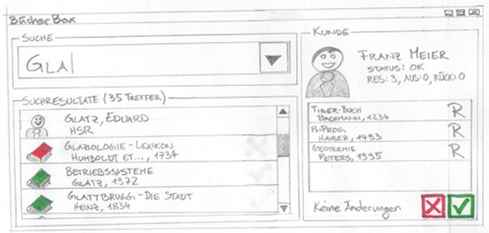
\includegraphics[width=45mm]{prototyp3Thumbnail} \\
   Prot. 3, Benutzeransicht
  \end{center}
\end{wrapfigure}

Und noch etwas: Der Laserscanner funktioniert wie ein normales Eingabegerät. Wird ein Code mit dieser Methode eingelesen, sollte dieser nicht an das Ende des Suchtextes angehängt werden. Ist man im Ausleihemodus, sollte der Suchtext unverändert bleiben, wenn man einen Buchcode einscannt.

\subsection{Prototyp 4 - 14.10.2009} 
\begin{wrapfigure}{r}{45mm}
  \begin{center}
   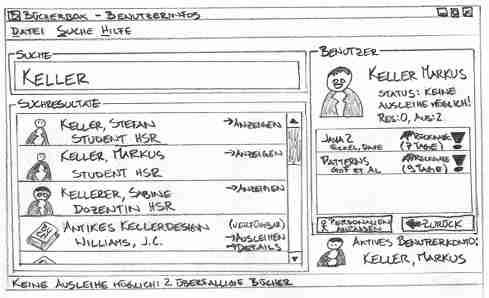
\includegraphics{prototyp4Thumbnail} \\
   Prot. 4, Benutzer mit Mahnungen
  \end{center}
\end{wrapfigure}
Auf das Feedback eines Projektbetreuers hin, dass der Status des Systemes nicht gut sichtbar ist, wurde in der rechten unteren Ecke ein Informationsfeld hinzugefügt, welches den zur Zeit aktiven Benutzer anzeigt. Das Kuchendiagramm auf dem Hauptbildschirm, welches über den Zustand der Bibliothek informiert wurde entfernt, da nicht interessant im täglichen Gebrauch. Neu ist zudem die Menüleiste, welche den Lernprozess unterstützen soll.

Ein weiterer Nebenprototyp wurde verworfen. Es wurde versucht, im unteren Teil des Userinterfaces eine Detailanzeige einzufügen, so dass das Fenster zu einem Quadrat wurde. Dies hätte jedoch die Übersichtlichkeit der Benutzeroberfläche beeinträchtigt und zudem sind moderne Bildschirme eher breit als hoch.

\subsection{Prototyp 5 - 15.10.2009}
\begin{wrapfigure}{r}{45mm}
  \begin{center}
   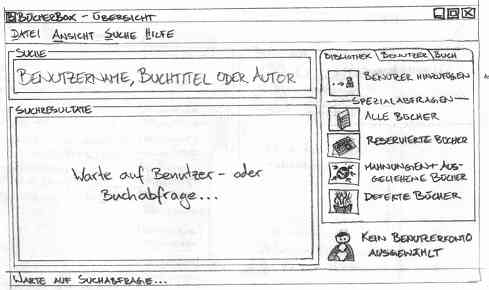
\includegraphics{prototyp5Thumbnail} \\
   Prot. 5, Übersicht
  \end{center}
\end{wrapfigure}
Der gestrige Prototyp wurde heute von einer echten Bibliothekarin der HSR getestet. Das Feedback ist in diesen neuen Prototypen eingeflossen. Verschiedene Beschriftungen wurden entfernt oder aus Verständlichkeitsgründen geändert. Es stellt sich heraus, dass die ''Zurück''-Buttons nicht verständlich sind. 
Als Gegenmassnahme wurden auf der rechten Seite Tabs eingeführt, welche über das aktuell ausgewählte Buch oder den letzten Benutzer Details anzeigen und es ermöglichen, wieder ins Hauptmenü zurückzukehren.

Interessant war ebenfalls, dass das produktive System der HSR-Bibliothek die Bücher beim Einscannen ohne weiteres Nachfragen zurückbucht. Das Vorgehen ist deshalb gefahrlos, da die Bibliothekarin das Buch ja in den Händen hält, es sich somit in der Bibliothek befindet. Der Klickaufwand wird so enorm minimiert. Es wird versucht, diesen Ablauf in das Miniprojekt einzubauen, wenn eine Bücher-ID gescannt oder getippt wird. Für Demonstrationszwecke wird es trotzdem nötig sein, dass man nach einem Buchtitel suchen kann und diesen ausleihen oder reservieren kann.

\subsection{Prototyp 6 - 16.10.2009}
\begin{wrapfigure}{r}{45mm}
  \begin{center}
   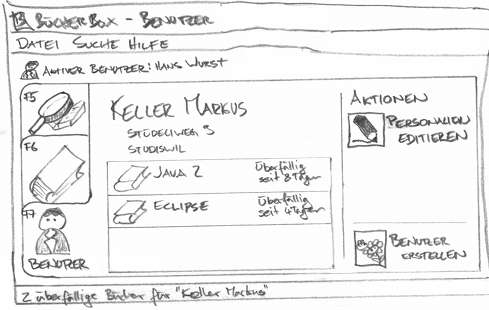
\includegraphics{prototyp6Thumbnail} \\
   Prot. 6, Benutzeransicht
  \end{center}
\end{wrapfigure}
Der Projektbetreuer hält folgende Punkte fest: Der Status des aktiven Benutzers ist zu wichtig, um ihn in die rechte untere Ecke zu drängen. Besser wäre, ihn rechts oder links oben zu platzieren. Zudem sind die Tabs auf der rechten Seite klein, um alle wichtigen Aktionen darin ausführen zu können. 
Während des Gesprächs hat sich herausgestellt, dass das Suchfenster ohne weiteres in einen Tab ausgelagert werden könnte. Damit wäre das Platzproblem für die Aktionen gelöst. 

Der neue Prototyp hat immer noch 3 Tabs, die jetzt auf der linken Seite platziert und mit einem Bild und einem Accelerator versehen wurden. Der ''Bibliothek''-Tab wurde umgewandelt in einen ''Recherche''-Tab und die Spezialsuchabfragen sind in einer Spalte auf der rechten Seite aufgelistet. Am linken oberen Rand des Fensters prangt neu das Feld mit dem aktiven Benutzer. Eine Schwierigkeit wird jetzt sein, den Übergang von der Recherche zu den Buchdetails mit möglichst wenig Aufwand zu gestalten.

\subsubsection{Review 23.10.2009}
Dank dem Review konnten drei weitere Punkte verbessert werden. Das ''X''-Bild beim defekten Buch sieht aus wie ein Button. Er wird deshalb ersetzt durch ein Durchstreichen des Buchtitels und einem kleineren Kreuz-Symbol neben dem Text zum Zustand. Als zweites war das zur Zeit gewählte Buch nicht ersichtlich, weshalb bei der TabbedPane ein ToolTip eingeblendet wird mit dem Titel des ausgewählten Buches. Zuletzt sollten im ''Aktionen''-Bereich mehr Knöpfe vorhanden sein, wie zum Beispiel ''Buch suchen'' oder ''Neue Suchanfrage''.

\section{Resultate}
\subsection{MUSS-Kriterien}
Die Muss-Kriterien wurde alle implementiert. Die Anzeige der Statistik wurde in der rechten unteren Ecke im Status-Panel untergebracht mit einem ausführlicheren Tooltip-Text.

Die Applikation ist durchgehend mit Mnemonics und Tastaturkürzeln ausgestattet. Die gegebenen Szenarien lassen sich per Tastatur auf verschiedene Arten durchgehen. Jede Aktion ist durch die Menüleiste und durch das Aktionspanel auf mindestens zwei Arten erreichbar. Im Folgenden werden die beiden vorgegebenen Szenarien per Tastatur durchgespielt:

\subsection{Szenario 1} Der Benutzer ''Jenni, Heinrich'' wurde für die Abgabe speziell präpariert, damit er abgelaufene Ausleihen besitzt und das erste Szenario ausprobiert werden kann. Die Suche nach dem Benutzer erfolgt durch Eingabe seines Namens in der Suchleiste. Ist der Benutzer eindeutig, so kann mit der Eingabetaste direkt zu seinen Ausleihen gewechselt werden. Falls nicht, wird der Fokus mit TAB auf die Suchresultate gewechselt und die Auswahl erfolgt mit den Pfeiltasten und der Eingabetaste. Jetzt werden die Benutzerdetails und die Ausleihen von Herrn Jenni angezeigt. Mit der Tabulatortaste kommt der Benutzer in die Liste mit den Ausleihen. Sobald eine bestimmte Ausleihe markiert ist, kann das betroffene Buch mit ''alt-z'' in die Bibliothek zurückgebracht werden. Wurden die beiden abgelaufenen Bücher zurückgegeben, ist der Benutzer nicht mehr gesperrt und der/die BibliothekarIn gelangt durch Drücken von F5 zur Suche. Dort kann er/sie die drei Bücher nacheinander eintippen, auswählen und in der Buchansicht mit ''alt-l'' ausleihen.

\subsection{Szenario 2} Bei der Buchrückgabe wird der Buchtitel eingetippt, das gewünschte Buch mit TAB und Eingabetaste ausgewählt und in der Buchansicht mit ''alt-z'' zurückgegeben. Ist ein Buch beschädigt, können die Defekte im Editiermodus (''alt-e'') eingetragen werden. Die Änderungen können mit der Eingabetaste oder ''strg-s'' bestätigt werden. Soll ein Buch ausgemustert werden, kann es mit ''alt-m'' markiert werden. Ein Dialog fragt, ob eine Rechnung gedruckt werden soll. ''alt-d'' lässt die Rechnung drucken (nicht implementiert). Danach kann das Buch nicht mehr ausgeliehen werden und es wird entsprechend gekennzeichnet.

\subsection{Benutzung des Observer-Patterns}
Die Filterung der Suchresultate erfolgt nicht mit dem von Swing bereitgestellten RowFilter sondern wurde selbst implementiert. Bei der Eingabe von Zeichen werden die Suchresultate dem Suchtext angepasst, was mit dem Observer-Pattern umgesetzt wurde. Das im Anhang abgebildete Sequenzdiagramm visualisiert den Vorgang bei der Initialisierung und bei der Eingabe von Zeichen. Ändern sich Daten in der Bibliothek, werden die Änderungen in der Resultateliste ebenfalls angezeigt (Verbindung mit Library, ganz rechts im Diagramm).

\subsection{KANN-Kriterien}
Von den optionalen Kriterien wurden die Bücher- und Benutzerverwaltung umgesetzt. Zudem wurden folgende Features eingebaut:
\begin{itemize}
	\item Statuszeile mit statischen und temporären Mitteilungen
	\item Splash-Screen, mit Hilfe der Manifest-Datei eingebunden
	\item Sortierung der Suchresultate und Ausleihen
	\item Spezialisierte CellRenderer mit integrierten Buttons (ermöglichen Ausleihe, Rückgabe und auswahl des Benutzers mit einem Klick)
	\item Konsequente Verwendung von Bildern für alle Aktionen
\end{itemize}

\section{Fazit und Erkenntnisse}
Es lohnt sich, die \textbf{Papierprototypen sorgfältig} zu \textbf{testen} und mit den Betreuern und Aussenstehenden zu besprechen. Die Tatsache, dass die Editier-Funktion nicht in die Papierprototypen eingebunden wurde, hat im späteren Verlauf zu einigen Schwierigkeiten geführt. Zudem sollte der Aufwand für eine benutzerfreundliche Implementation nicht unterschätzt werden. Scheinbar einfache Elemente wie eine eigene FocusTraversalPolicy können viel Zeit benötigen wenn sie nicht gleich auf Anhieb funktionieren.

Ein schwieriges Thema ist die \textbf{Wahl der Architektur} bei der GUI-Programmierung. Es wurden verschiedene Lösungen betrachtet, wie die einzelnen Komponenten ihre Daten untereinander austauschen. In der entwickelten Applikation findet dieser Austausch über eine Model-Verwaltung statt, welche Zugriff bietet auf alle Models. Eine Referenz zu dieser Verwaltung wird jedem grafischen Element mitgegeben. Eine elegantere Lösung könnte die Verwendung eines Business-Layers darstellen. Dabei wird das gesamte Verhalten in den Business-Layer gepackt und die grafischen Elemente dienen wirklich nur noch zur Darstellung. Eine solche Lösung könnte auch besser automatisiert getestet werden. Eine interessante Alternative könnte auch das MVP-Pattern bieten, welches von Martin Fowler in einem Dokument namens ''GUI Architectures'' diskutiert wird. Es wird dort ein \textit{Presentator} eingesetzt, welcher die gesamten grafischen Elemente mit den unteren Schichten verknüpft.

\includepdf[landscape=true]{Guimap.pdf}
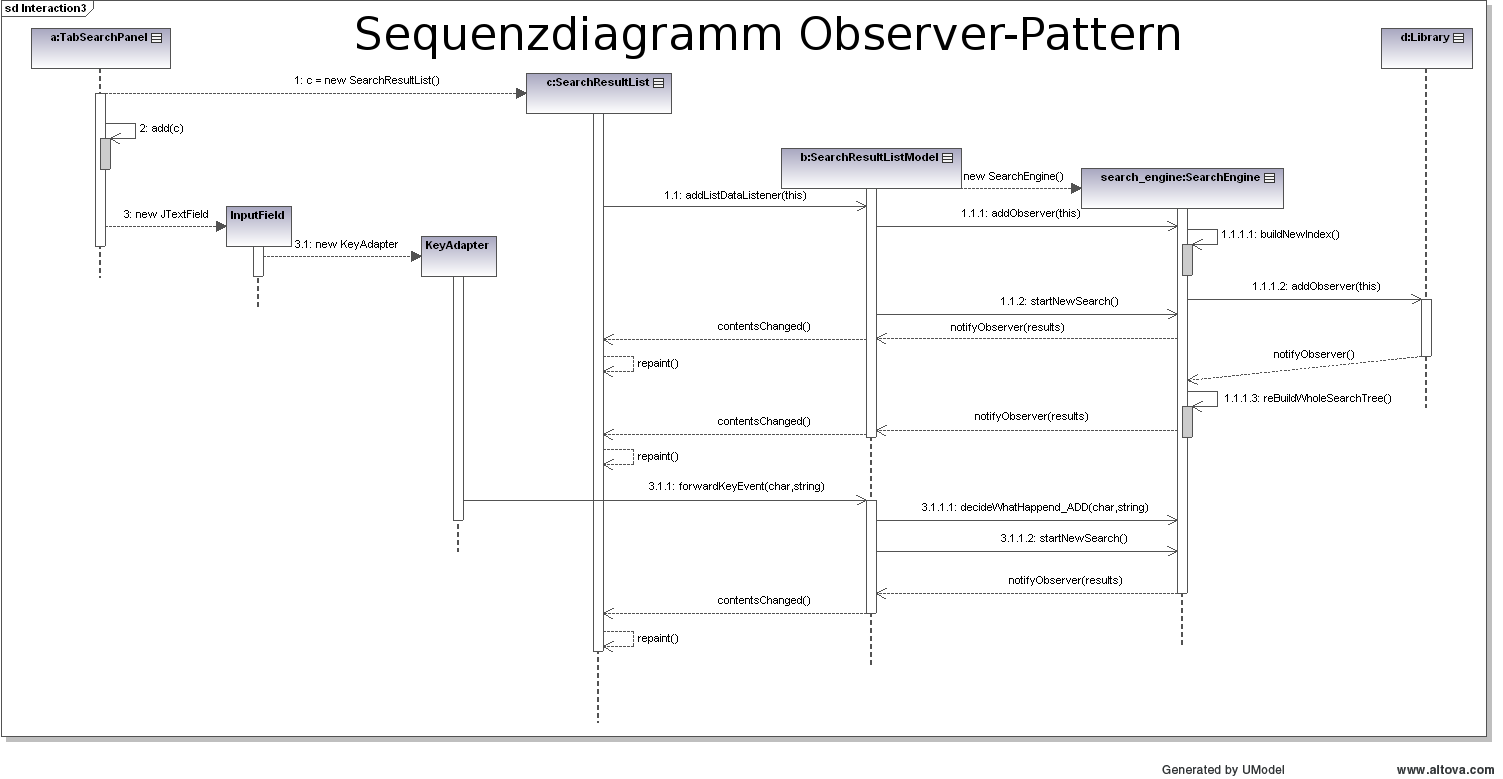
\includepdf[landscape=true]{SequenzDiagramObserver.png}
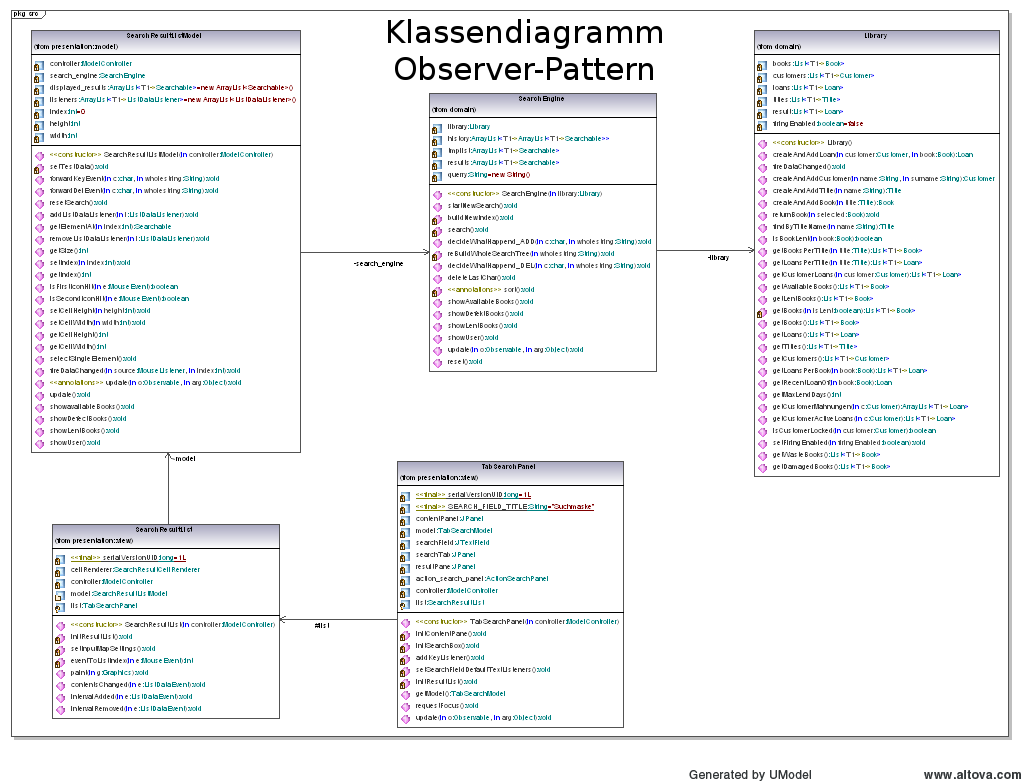
\includepdf[landscape=true]{ClassDiagramObserver.png}

\end{document}


